\section{Préhenseur}

Un préhensue rest requis afin de soulever le trésor et l'amener à destination. Afin d'économiser la charge du condensateur, il faut miniser le temps requis où l'électroaimant est allumé. Il est donc optimal de soulever le trésor à l'horizontale, dans une position où il repose sur une surface plate. 

Pour ce faire, le préhenseur est constitué d'un arbre entrainé par un servo-moteur controllé par le pollulu, comme visible sur la figure \ref{fig:lift_down}. l'électroaimant destiné à prendre le trésor est fixé au milieu de l'arbre. Lorsqu'un trésor est pris par le préhenseur, il est soulevé puis bascullé contre un muret de bois comme sur la figure \ref{fig:lift_up}. Il est alors possible de conserver le trésor sans qu'aucune puissance ne soit consommé.

\begin{figure}[ht]
  \centering
  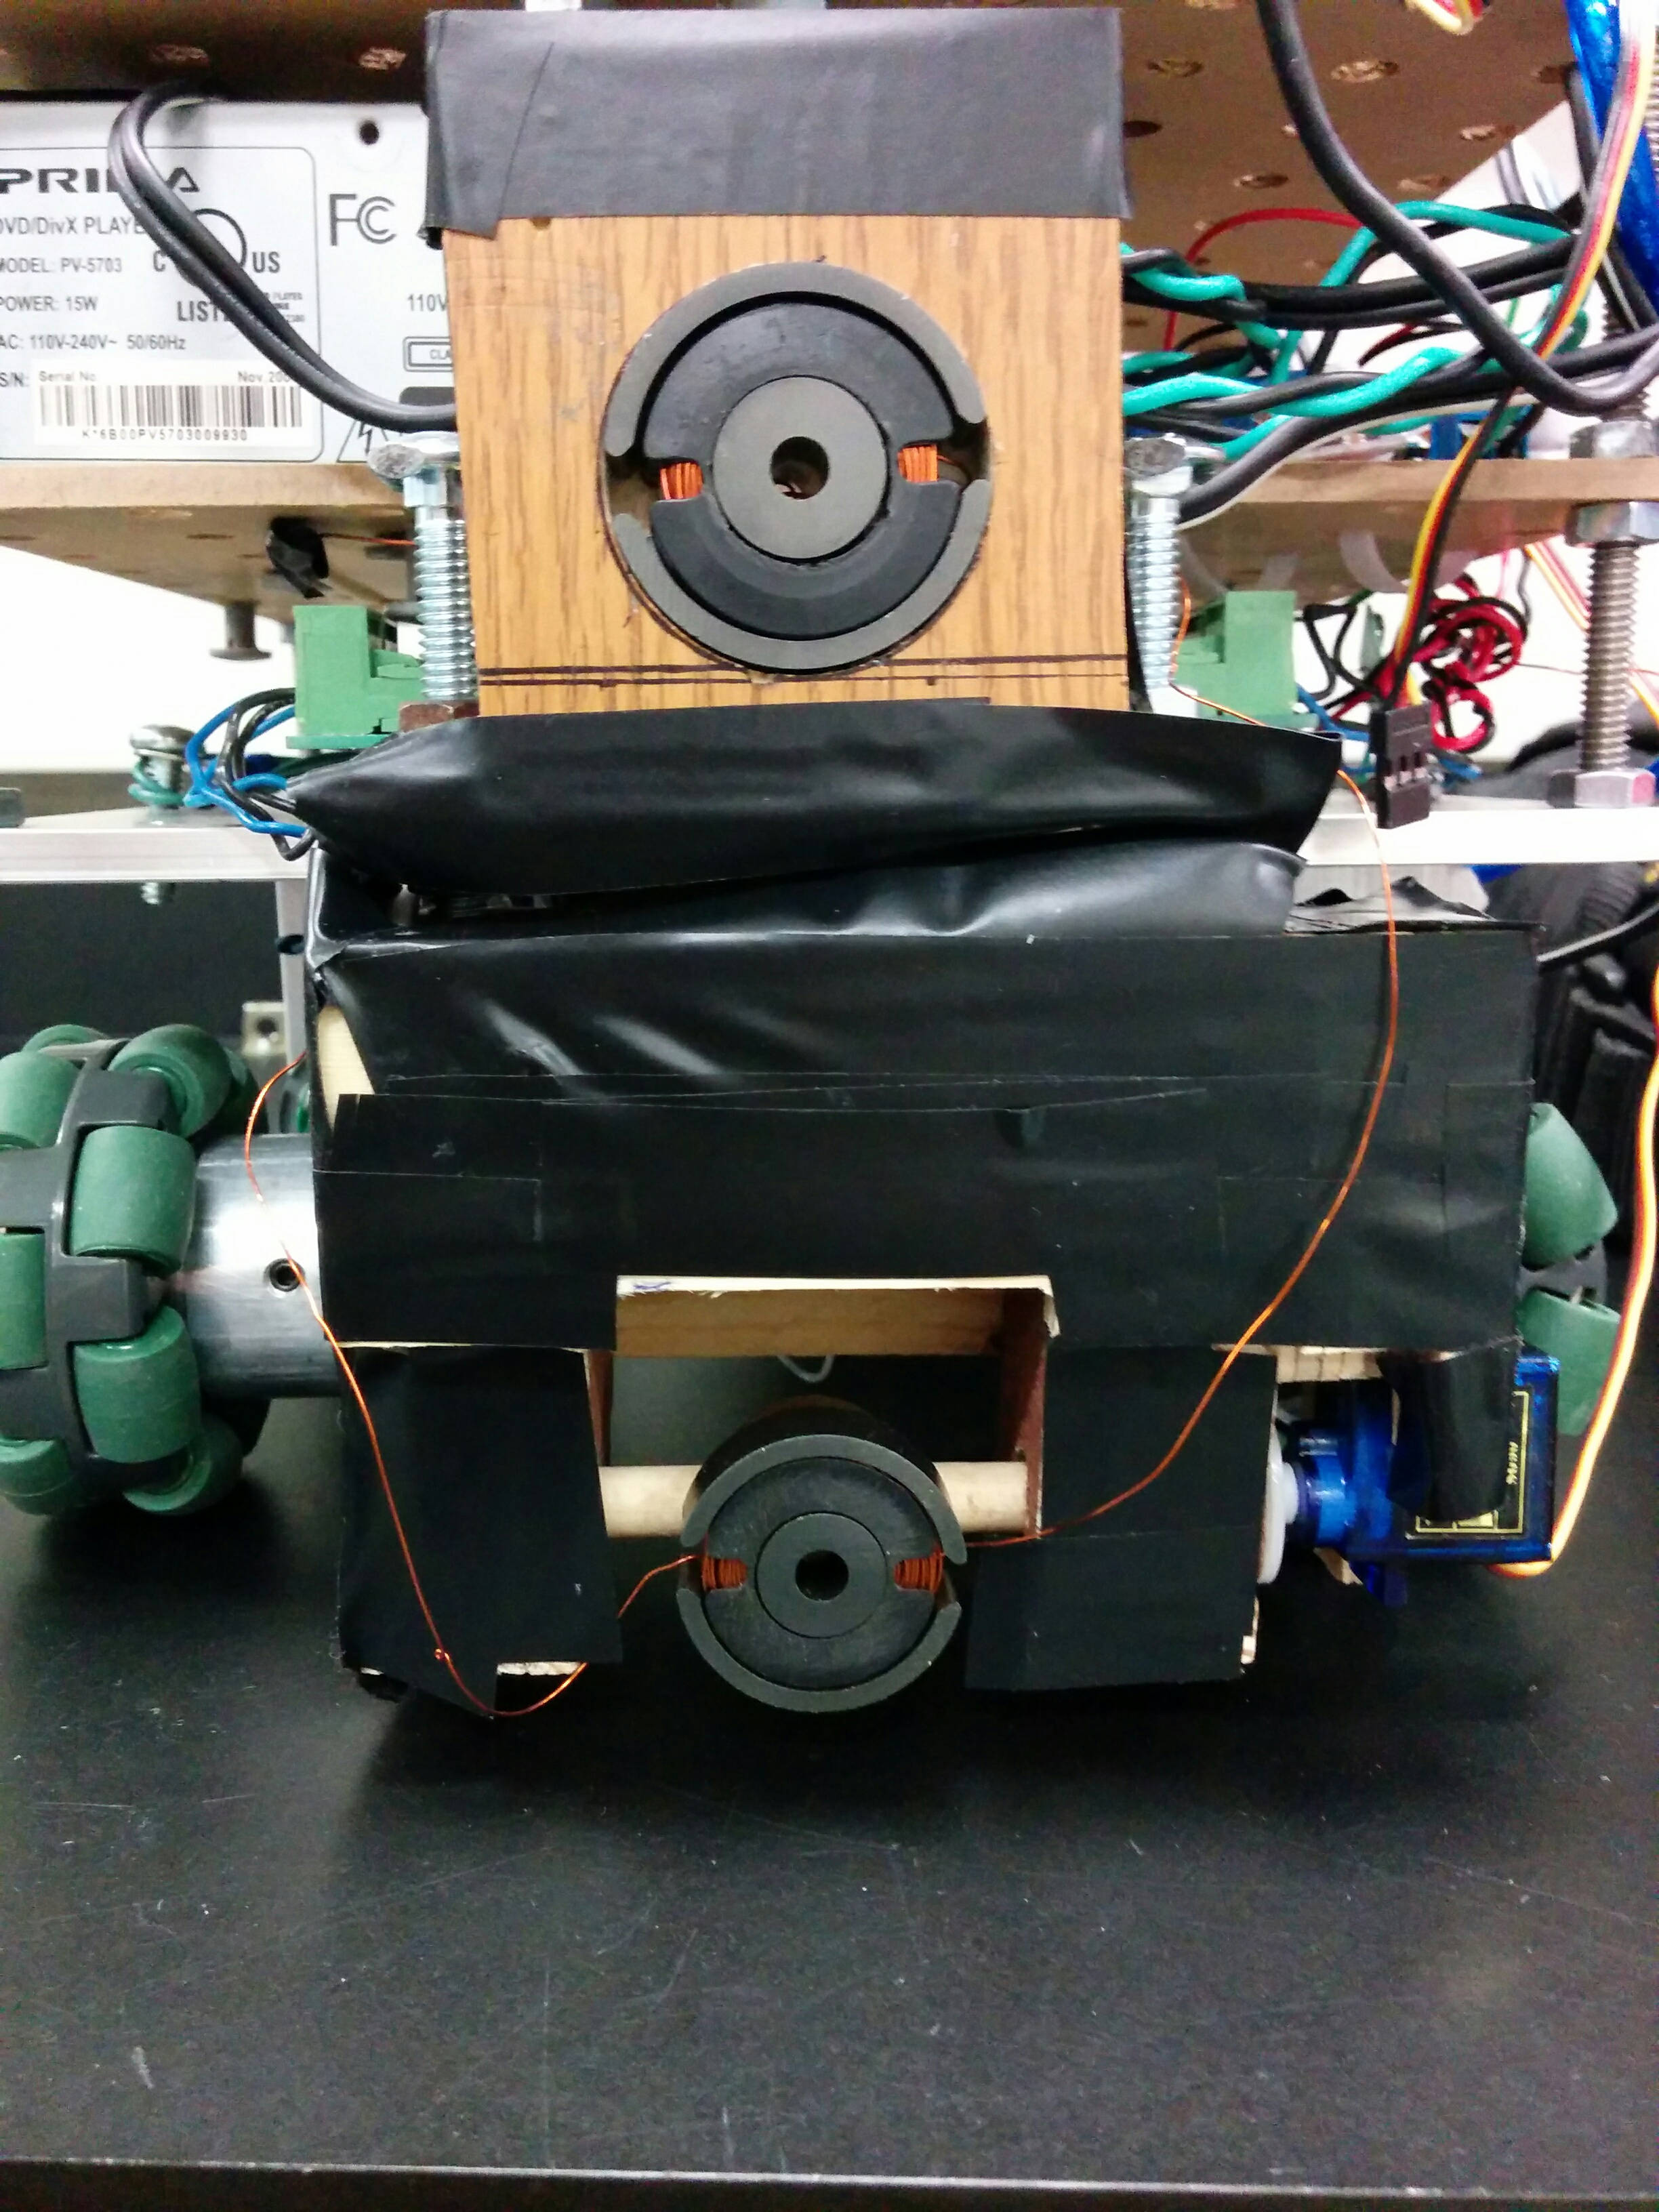
\includegraphics[scale=0.05]{resources/prehenseur_down.jpg}
  \caption{préhenseur en position de prise de trésor}
  \label{fig:lift_down}
\end{figure}

\begin{figure}[ht]
  \centering
  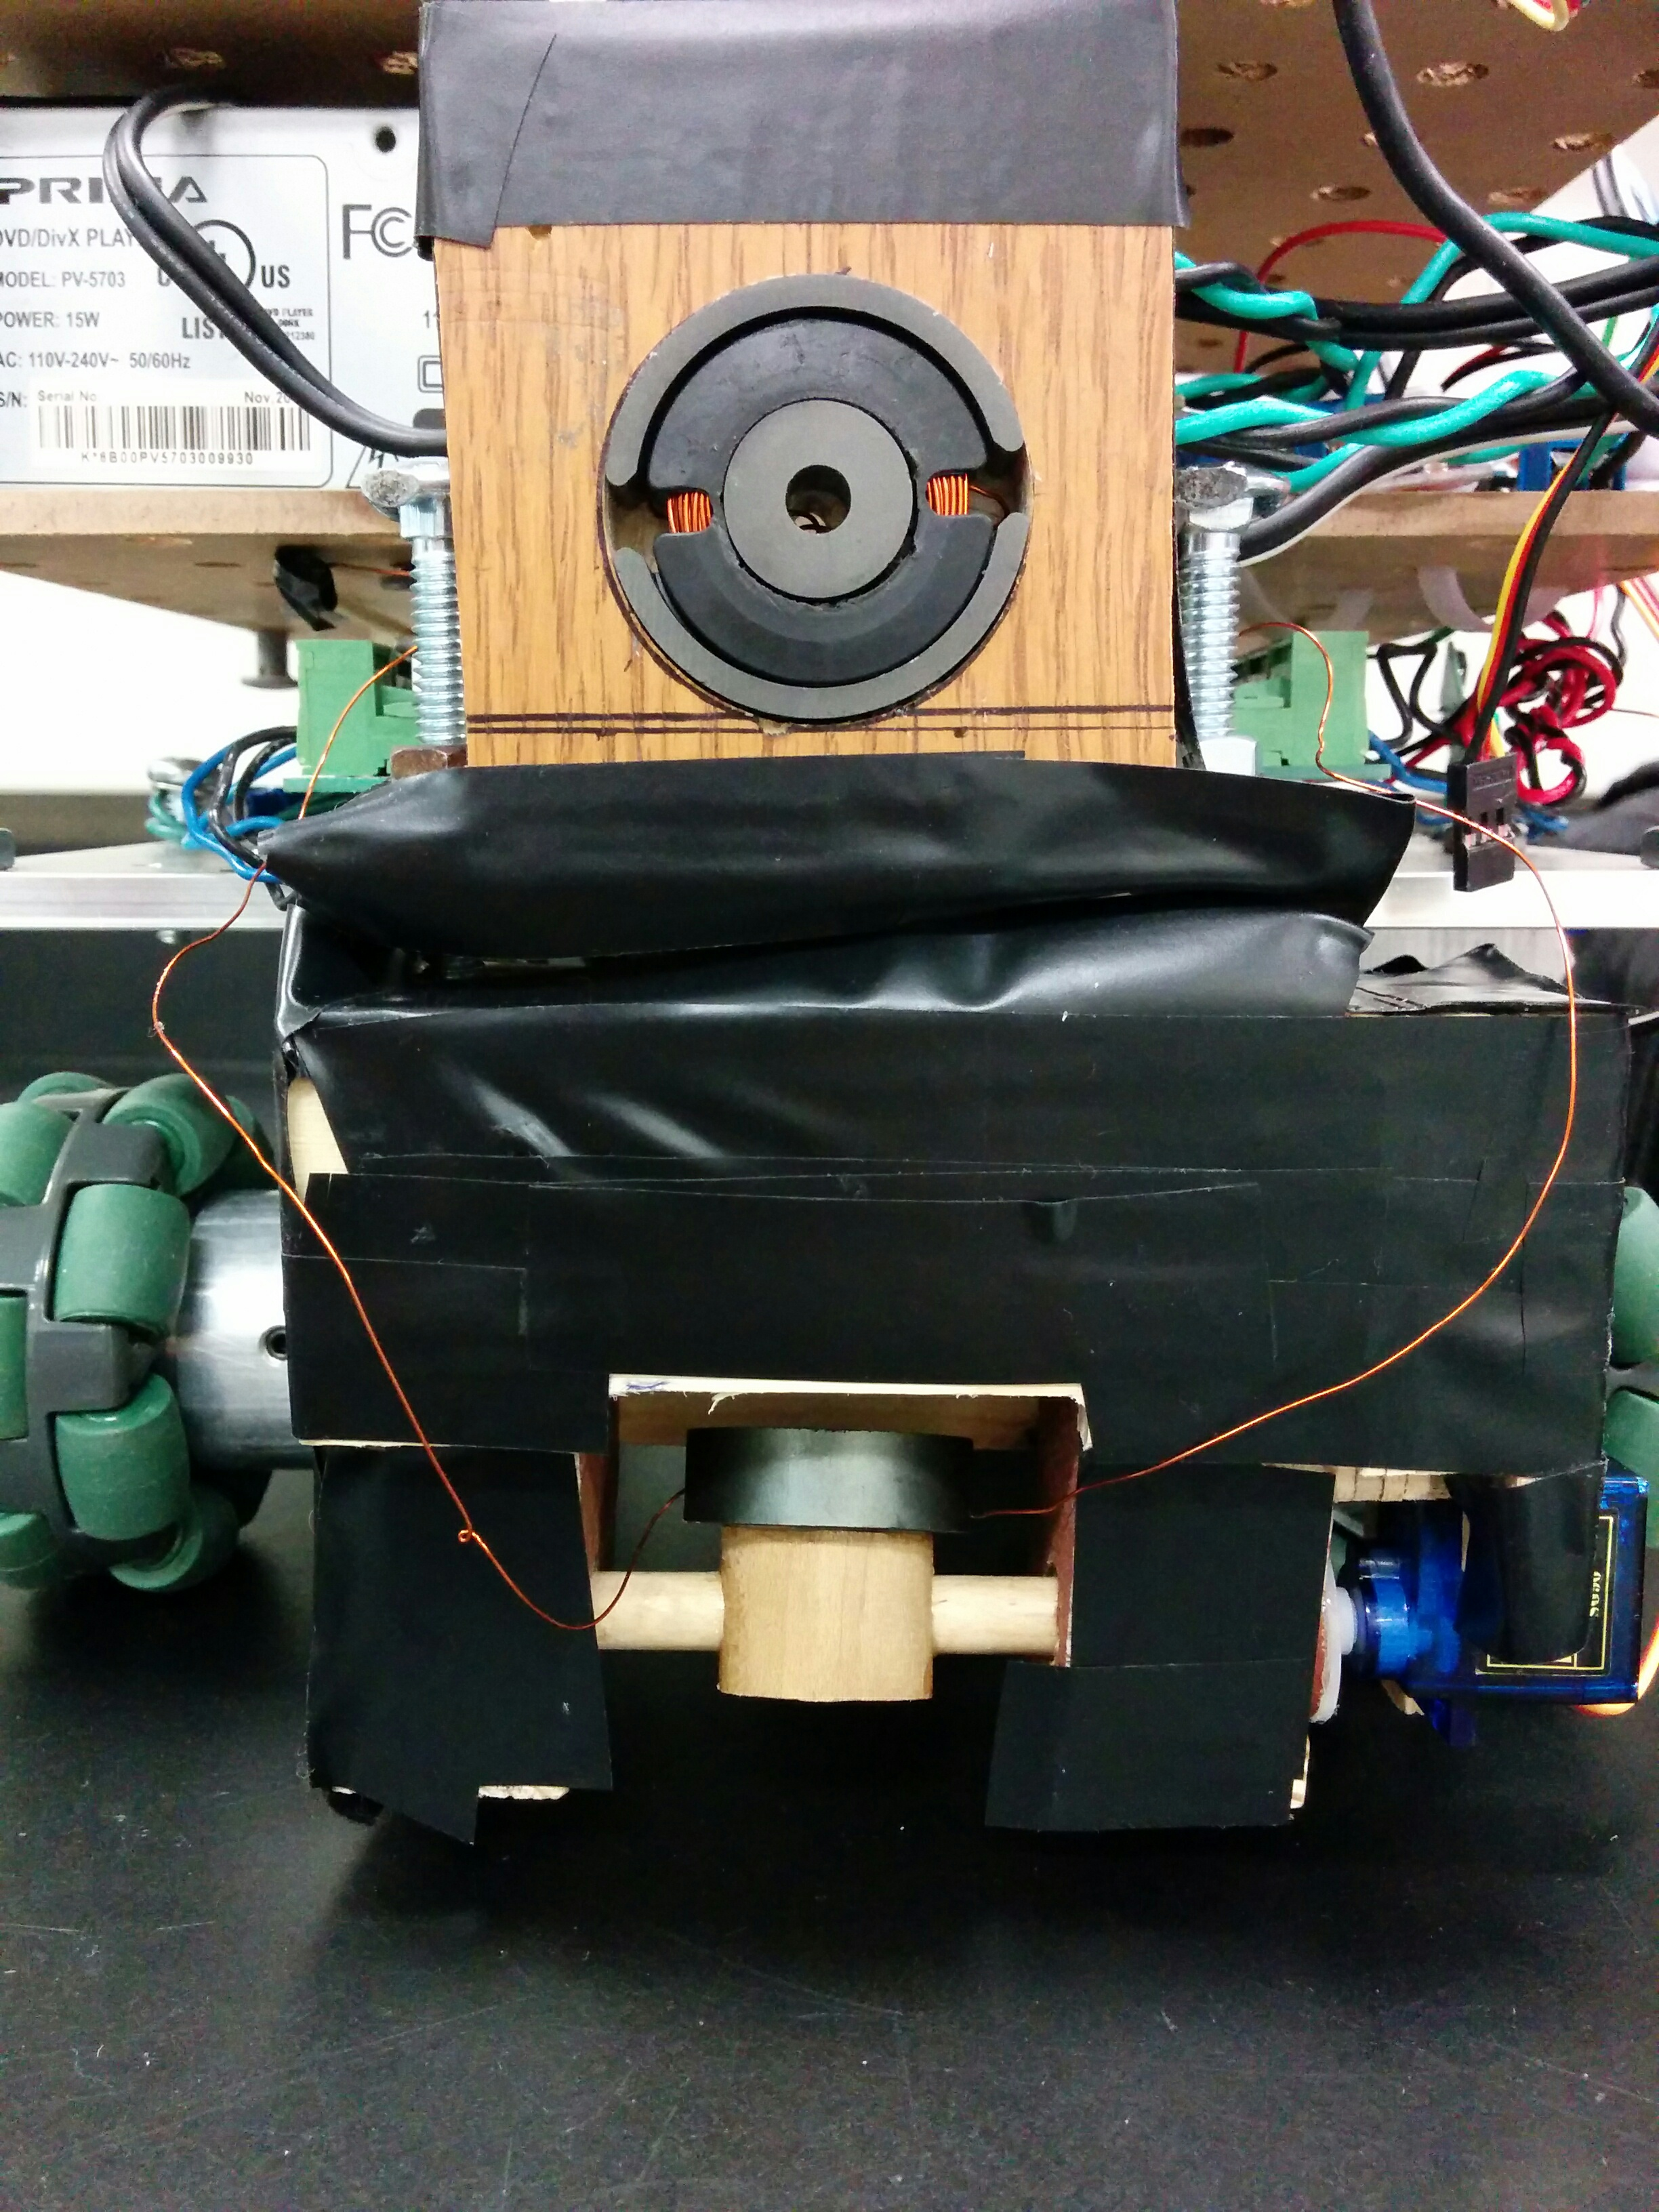
\includegraphics[scale=0.05]{resources/prehenseur_up.jpg}
  \caption{préhenseur en position de conservation du trésor}
  \label{fig:lift_up}
\end{figure}
